% Provenance (never printed): cycle 2 "Questionner le monde de la matiere"
% (solid materials, observing and sorting) and cycle 3 theme 4 (local geology,
% rocks for building); see sources/book1/PROVENANCE.md. Book 1, grade 3, ch. 1.
\chapter{Batu, Kerakal, dan Pasir}\label{ch:g3:stones-pebbles-sand}

Tom sedang berlibur di tepi \omterm{def:g1:landscapes-around-us:water}{sungai}. Di gosong berkerikil, tempat airnya
dangkal, ia memungut sebutir \omterm{def:g3:stones-pebbles-sand:pebble}{kerakal}. \omterm{def:g3:stones-pebbles-sand:pebble}{Kerakal} itu licin dan bulat, hampir
seperti telur, dan pas di genggamannya. Minggu lalu, ketika berjalan
bersama orang tuanya di jalan setapak \omterm{def:g1:landscapes-around-us:landform}{gunung} jauh di hulu \omterm{def:g1:landscapes-around-us:landform}{lembah} yang sama,
ia melihat batu-batu berwarna sama tergeletak di bawah lereng berbatu ---
tetapi batu-batu itu tajam, bersudut dan bertepi.

Bagaimana sebuah batu tajam dari \omterm{def:g1:landscapes-around-us:landform}{gunung} bisa menjadi \omterm{def:g3:stones-pebbles-sand:pebble}{kerakal} yang licin dan
bulat di bawah sana, di \omterm{def:g1:landscapes-around-us:landform}{lembah}? Untuk mengetahuinya, mari kita mulai dari
\omterm{def:g3:stones-pebbles-sand:rock}{batuannya} sendiri.

\begin{omfigure}
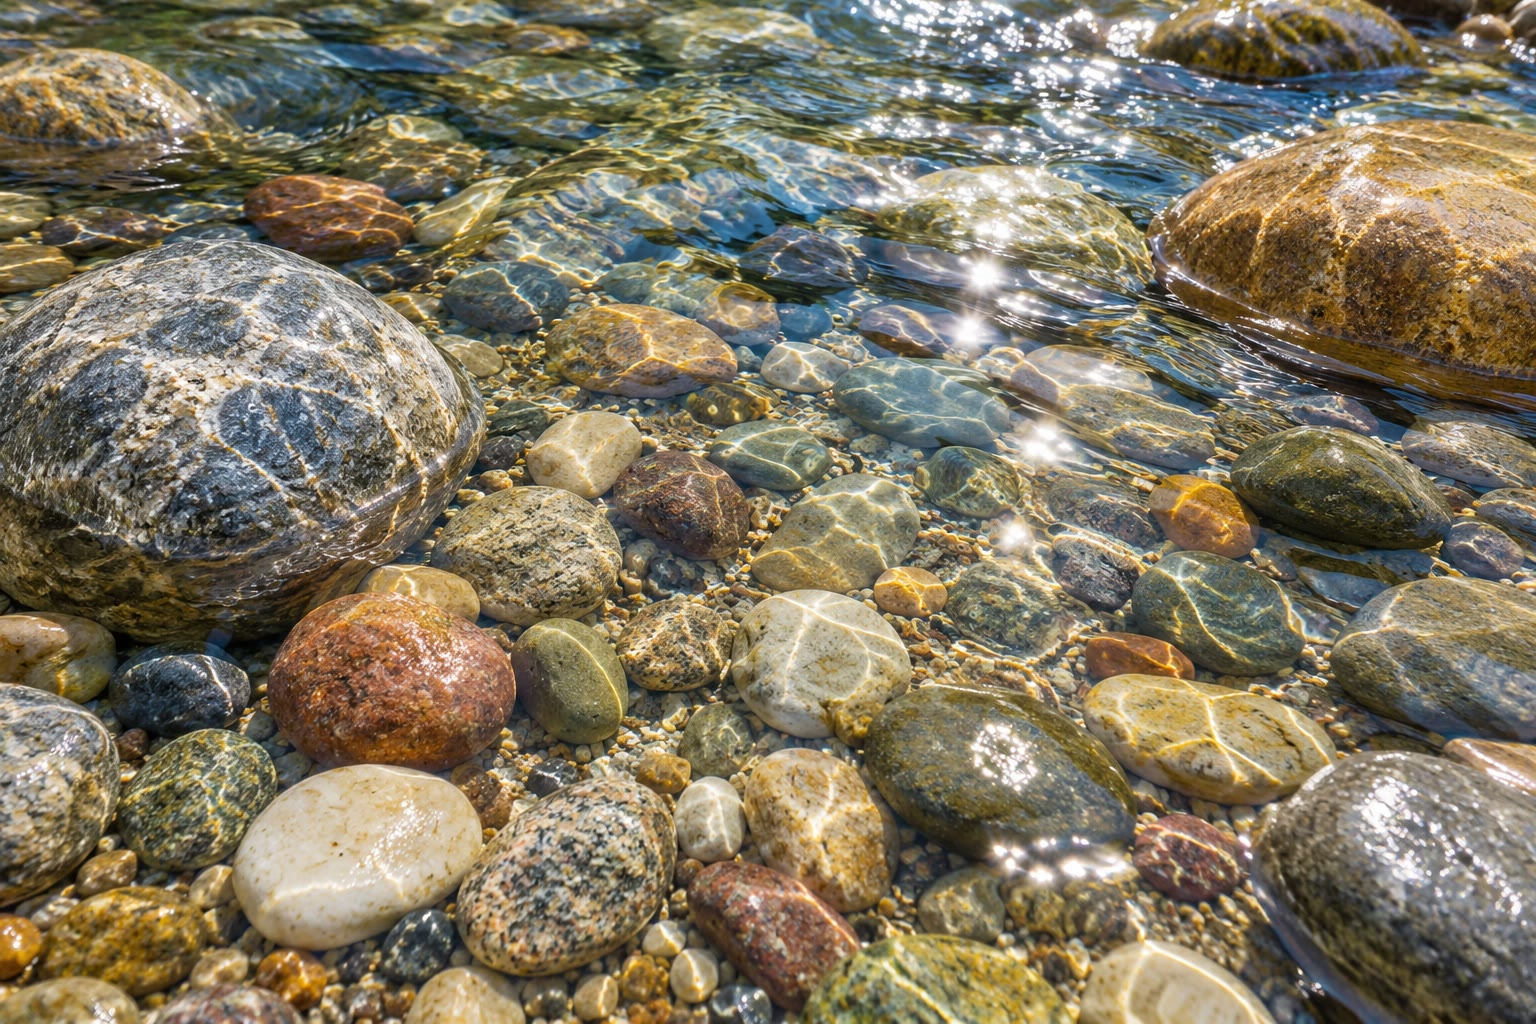
\includegraphics[width=0.62\linewidth]{images/book1/ai/g3-stream-pebbles.jpg}

{\small \omterm{def:g3:stones-pebbles-sand:pebble}{Kerakal-kerakal} bulat di bawah air jernih sebuah \omterm{def:g1:landscapes-around-us:water}{sungai} kecil.}
\end{omfigure}

\begin{recall}
Dalam \omterm{def:g1:landscapes-around-us:landscape}{bentang alam} ada \omterm{def:g1:landscapes-around-us:landform}{gunung}, \omterm{def:g1:landscapes-around-us:landform}{bukit}, \omterm{def:g1:landscapes-around-us:landform}{lembah}, dan \omterm{def:g1:landscapes-around-us:landform}{dataran}, serta \omterm{def:g1:landscapes-around-us:water}{sungai} yang
mengalir dari daratan tinggi turun ke \omterm{def:g2:water-on-earth:ocean}{laut}
(\cref{ch:g1:landscapes-around-us}). Lapisan tanah paling atas, tempat
tumbuhan tumbuh, adalah tanah: buku biologi menceritakan bagaimana makhluk
hidup membentuknya.
\end{recall}

\section{Batuan: tanah keras di bawah kaki kita}

Galilah lubang yang dalam di sebuah kebun. Mula-mula kamu menemukan tanah
yang gelap dan lunak, berisi akar. Di bawahnya, tanah menjadi lebih terang
warnanya dan lebih berbatu. Dan jika kamu bisa menggali cukup dalam, kamu
selalu akan sampai pada sesuatu yang keras yang tidak bisa dipotong sekop:
\omterm{def:g3:stones-pebbles-sand:rock}{batuan}.

\begin{definition}[Batuan dan batuan dasar]\label{def:g3:stones-pebbles-sand:rock}
Yang disebut \emph{batuan}\index{batuan} adalah bahan alami yang keras,
penyusun Bumi yang padat. Yang disebut \emph{batuan dasar}\index{batuan dasar}
adalah batuan padat yang terletak di bawah tanah di semua tempat di daratan,
dan di bawah \omterm{def:g3:stones-pebbles-sand:sand}{pasir} dan \omterm{def:g3:stones-pebbles-sand:sand}{lumpur} dasar \omterm{def:g2:water-on-earth:ocean}{laut}.
\end{definition}

Di kebanyakan tempat, \omterm{def:g3:stones-pebbles-sand:rock}{batuan dasar} tersembunyi di bawah tanah, rumput, dan
pepohonan. Kita melihatnya di tempat yang tidak ada tanah yang menutupinya:
di sisi \omterm{def:g1:landscapes-around-us:landform}{gunung} yang curam, di tebing di tepi \omterm{def:g2:water-on-earth:ocean}{laut}, dan di sepanjang jalan
yang dibangun dengan memotong \omterm{def:g1:landscapes-around-us:landform}{bukit}.

\begin{omfigure}
\begin{tikzpicture}[x=1cm, y=1cm, font=\small]
  % bedrock
  \fill[omLithGranite!60] (0,0) rectangle (11,2.2);
  \foreach \x/\y in {0.6/0.5, 1.8/1.4, 3.1/0.7, 4.4/1.6, 5.6/0.4, 6.9/1.2, 8.3/0.6, 9.6/1.5, 10.3/0.4}
    \draw[black!40, line width=0.4pt] (\x,\y) -- ++(0.5,0.25);
  % soil (thick on the left, missing on the steep right)
  \fill[brown!55] (0,2.2) -- (0,3.4) .. controls (2,3.5) and (4,3.4) .. (5.6,3.2) -- (6.4,2.9) -- (6.4,2.2) -- cycle;
  \fill[brown!30] (0,2.2) rectangle (6.4,2.65);
  % rock showing on the right: a hill side with no soil
  \fill[omLithGranite!60] (6.4,2.2) -- (6.4,2.9) -- (7.6,3.9) -- (8.8,4.3) -- (11,4.3) -- (11,2.2) -- cycle;
  \draw[black!60] (0,3.4) .. controls (2,3.5) and (4,3.4) .. (5.6,3.2) -- (6.4,2.9) -- (7.6,3.9) -- (8.8,4.3) -- (11,4.3);
  % grass and roots
  \foreach \x in {0.3,0.8,...,5.3}
    \draw[green!50!black, line width=0.6pt] (\x,{3.4-0.04*\x}) -- ++(0.05,0.18);
  \foreach \x in {1.2,3.4,4.9}
    \draw[brown!80!black, line width=0.5pt] (\x,3.3) -- ++(-0.1,-0.5) -- ++(0.15,-0.3);
  % labels
  \node[anchor=west] at (11.2,3.6) {batuan yang tampak};
  \node[anchor=west] at (11.2,3.2) {di permukaan};
  \draw[black!60] (11.15,3.4) -- (9.6,4.15);
  \node[anchor=east] at (-0.2,2.9) {tanah};
  \draw[black!60] (-0.15,2.9) -- (0.6,2.9);
  \node[anchor=west] at (11.2,1.1) {batuan dasar};
  \draw[black!60] (11.15,1.1) -- (10.6,1.1);
\end{tikzpicture}

{\small Penampang tanah. Di bawah tanah selalu ada \omterm{def:g3:stones-pebbles-sand:rock}{batuan dasar} yang padat.
Di lereng \omterm{def:g1:landscapes-around-us:landform}{bukit} yang curam, di sebelah kanan, tanahnya tidak ada dan
\omterm{def:g3:stones-pebbles-sand:rock}{batuannya} tampak di permukaan.}
\label{fig:g3:stones-pebbles-sand:ground}
\end{omfigure}

\section{Dari batuan menjadi kerakal}

\omterm{def:g3:stones-pebbles-sand:rock}{Batuan} itu keras, tetapi tidak bertahan selamanya. Pada musim dingin, air
masuk ke retakan \omterm{def:g3:stones-pebbles-sand:rock}{batuan}, membeku dan memuai, lalu mendorong retakan itu
menjadi lebih lebar. Akar tumbuhan juga tumbuh masuk ke dalam retakan.
Sedikit demi sedikit, potongan-potongan \omterm{def:g3:stones-pebbles-sand:rock}{batuan} patah dan jatuh: dari
situlah datangnya batu-batu tajam di bawah lereng \omterm{def:g1:landscapes-around-us:landform}{gunung}.

Ketika sebuah batu tajam jatuh ke \omterm{def:g1:landscapes-around-us:water}{sungai} kecil di pegunungan, air
menggulingkannya di sepanjang dasar \omterm{def:g1:landscapes-around-us:water}{sungai}, membenturkannya ke batu-batu
lain, dan menyeretnya di atas \omterm{def:g3:stones-pebbles-sand:sand}{pasir}. Sudut-sudutnya yang pertama-tama aus.
Makin jauh batu itu terbawa, makin bulat dan makin licin jadinya. Ketika
sampai di \omterm{def:g1:landscapes-around-us:landform}{lembah} bagian bawah, batu itu sudah menjadi \omterm{def:g3:stones-pebbles-sand:pebble}{kerakal}.

\begin{definition}[Kerakal dan kerikil]\label{def:g3:stones-pebbles-sand:pebble}
Yang disebut \emph{kerakal}\index{kerakal} adalah potongan kecil \omterm{def:g3:stones-pebbles-sand:rock}{batuan} yang
sudah dibulatkan dan dihaluskan oleh air yang menggulingkannya, di \omterm{def:g1:landscapes-around-us:water}{sungai}
atau di pantai. Yang disebut \emph{kerikil}\index{kerikil} adalah kumpulan
batu kecil dan kerakal yang terletak bersama-sama, dengan butiran yang
lebih besar daripada butiran \omterm{def:g3:stones-pebbles-sand:sand}{pasir}.
\end{definition}

\begin{omfigure}
\begin{tikzpicture}[x=1cm, y=1cm, font=\small]
  \draw[ocBlue!70!black, line width=1.2pt, -{Stealth[length=3mm]}] (0,0) -- (12.2,0);
  \node[below, font=\scriptsize] at (6.1,-0.15) {sungai membawa batu itu menuruni lereng, sedikit lebih jauh pada setiap banjir};
  \foreach \x/\shape/\t in {
     0.8/{(-0.55,-0.1) -- (-0.2,0.5) -- (0.35,0.55) -- (0.6,0.05) -- (0.3,-0.45) -- (-0.35,-0.5) -- cycle}/jatuh dari batuan,
     4.0/{(-0.5,-0.1) [rounded corners=4pt] -- (-0.2,0.45) -- (0.3,0.5) -- (0.55,0.05) -- (0.3,-0.4) -- (-0.35,-0.45) -- cycle}/sudutnya aus,
     7.2/{(-0.45,-0.05) [rounded corners=8pt] -- (-0.15,0.42) -- (0.3,0.45) -- (0.5,0.05) -- (0.3,-0.35) -- (-0.3,-0.4) -- cycle}/lebih bulat dan lebih kecil,
     10.4/{(0,0) ellipse (0.45 and 0.3)}/kerakal yang licin} {
    \begin{scope}[shift={(\x,1.1)}]
      \fill[omLithGranite!80, draw=black!70] \shape;
    \end{scope}
    \node[font=\scriptsize] at (\x,0.35) {\t};
  }
\end{tikzpicture}

{\small Perjalanan sebuah batu di \omterm{def:g1:landscapes-around-us:water}{sungai}: tajam ketika jatuh dari \omterm{def:g3:stones-pebbles-sand:rock}{batuan},
bulat dan licin setelah perjalanan panjang ke hilir.}
\label{fig:g3:stones-pebbles-sand:journey}
\end{omfigure}

\begin{remark}[Membaca bentuk batu]\label{rem:g3:stones-pebbles-sand:shape}
Bentuk sebuah batu menceritakan kisahnya. Batu yang tajam belum menempuh
perjalanan jauh dari \omterm{def:g3:stones-pebbles-sand:rock}{batuan} asalnya. \omterm{def:g3:stones-pebbles-sand:pebble}{Kerakal} yang bulat dan licin sudah
lama digulingkan air, di \omterm{def:g1:landscapes-around-us:water}{sungai} atau oleh ombak \omterm{def:g2:water-on-earth:ocean}{laut}.
\end{remark}

\section{Pasir dan lumpur}

Batu dan \omterm{def:g3:stones-pebbles-sand:pebble}{kerakal} yang saling berbenturan juga melepaskan
serpihan-serpihan yang sangat kecil. Dalam waktu yang sangat lama,
serpihan-serpihan kecil ini menjadi \omterm{def:g3:stones-pebbles-sand:sand}{pasir}. Lihatlah \omterm{def:g3:stones-pebbles-sand:sand}{pasir} dengan kaca
pembesar: setiap butirnya adalah potongan kecil \omterm{def:g3:stones-pebbles-sand:rock}{batuan}, atau cangkang,
yang sering juga bulat.

\begin{definition}[Pasir dan lumpur]\label{def:g3:stones-pebbles-sand:sand}
% ledger: usgs:wentworth
Yang disebut \emph{pasir}\index{pasir} adalah butiran lepas pecahan \omterm{def:g3:stones-pebbles-sand:rock}{batuan}
yang lebih kecil daripada 2 milimeter: kita masih bisa melihat setiap
butirnya. Yang disebut \emph{lumpur}\index{lumpur} adalah butiran yang begitu
kecil sehingga kita tidak bisa melihatnya satu per satu; dalam keadaan
basah, lumpur lunak dan lengket.
\end{definition}

Para ahli geologi memilah pecahan \omterm{def:g3:stones-pebbles-sand:rock}{batuan} menurut ukurannya, dari yang
terbesar sampai yang terkecil: bongkah, \omterm{def:g3:stones-pebbles-sand:pebble}{kerakal} dan \omterm{def:g3:stones-pebbles-sand:pebble}{kerikil}, \omterm{def:g3:stones-pebbles-sand:sand}{pasir}, dan
\omterm{def:g3:stones-pebbles-sand:sand}{lumpur}.

\begin{omfigure}
\begin{tikzpicture}[x=1mm, y=1mm, font=\small]
  % true size: 1 unit = 1 mm
  \draw[black!40] (0,-14) -- (150,-14);
  \foreach \x in {0,10,...,150} \draw[black!40] (\x,-14) -- (\x,-12.5);
  \foreach \x in {0,50,100,150} \node[font=\scriptsize, below] at (\x,-14.5) {\pgfmathparse{int(\x/10)}\pgfmathresult\,cm};
  % mud: too small
  \node[font=\scriptsize, align=center] at (6,14) {lumpur};
  \fill[brown!60] (6,0) circle (0.05);
  \node[font=\scriptsize, align=center] at (6,4.5) {butiran terlalu\\kecil untuk dilihat};
  % sand grains: up to 2 mm
  \node[font=\scriptsize] at (28,14) {pasir};
  \foreach \x/\r in {22/0.3, 25/0.5, 28/0.75, 32/1.0}
    \fill[yellow!60!brown, draw=black!50, line width=0.2pt] (\x,0) circle (\r);
  \node[font=\scriptsize, align=center] at (28,5) {lebih kecil dari\\2 milimeter};
  % gravel and pebbles
  \node[font=\scriptsize] at (78,22) {kerikil dan kerakal};
  \fill[omLithGranite!80, draw=black!60] (52,0) ellipse (2 and 1.5);
  \fill[black!25, draw=black!60] (62,0) ellipse (4 and 3);
  \fill[omLithGranite!80, draw=black!60] (78,0) ellipse (8 and 6);
  \fill[black!30, draw=black!60] (104,0) ellipse (15 and 10);
  % boulder: off scale
  \node[font=\scriptsize] at (138,22) {bongkah};
  \fill[black!20, draw=black!60] (128,-10) .. controls (127,8) and (135,16) .. (142,15) .. controls (150,14) and (152,4) .. (149,-10) -- cycle;
  \node[font=\scriptsize, align=center, fill=white, fill opacity=0.7, text opacity=1, inner sep=1pt] at (139,4) {digambar jauh\\terlalu kecil};
\end{tikzpicture}

{\small Butiran pecahan \omterm{def:g3:stones-pebbles-sand:rock}{batuan} dari yang terkecil sampai yang terbesar.
\omterm{def:g3:stones-pebbles-sand:sand}{Lumpur}, \omterm{def:g3:stones-pebbles-sand:sand}{pasir}, \omterm{def:g3:stones-pebbles-sand:pebble}{kerikil}, dan \omterm{def:g3:stones-pebbles-sand:pebble}{kerakal} digambar dengan ukuran sebenarnya:
bandingkan dengan penggaris. Sebuah bongkah bisa sebesar kursi, atau
sebesar rumah.}
\label{fig:g3:stones-pebbles-sand:sizes}
\end{omfigure}

\begin{omfigure}
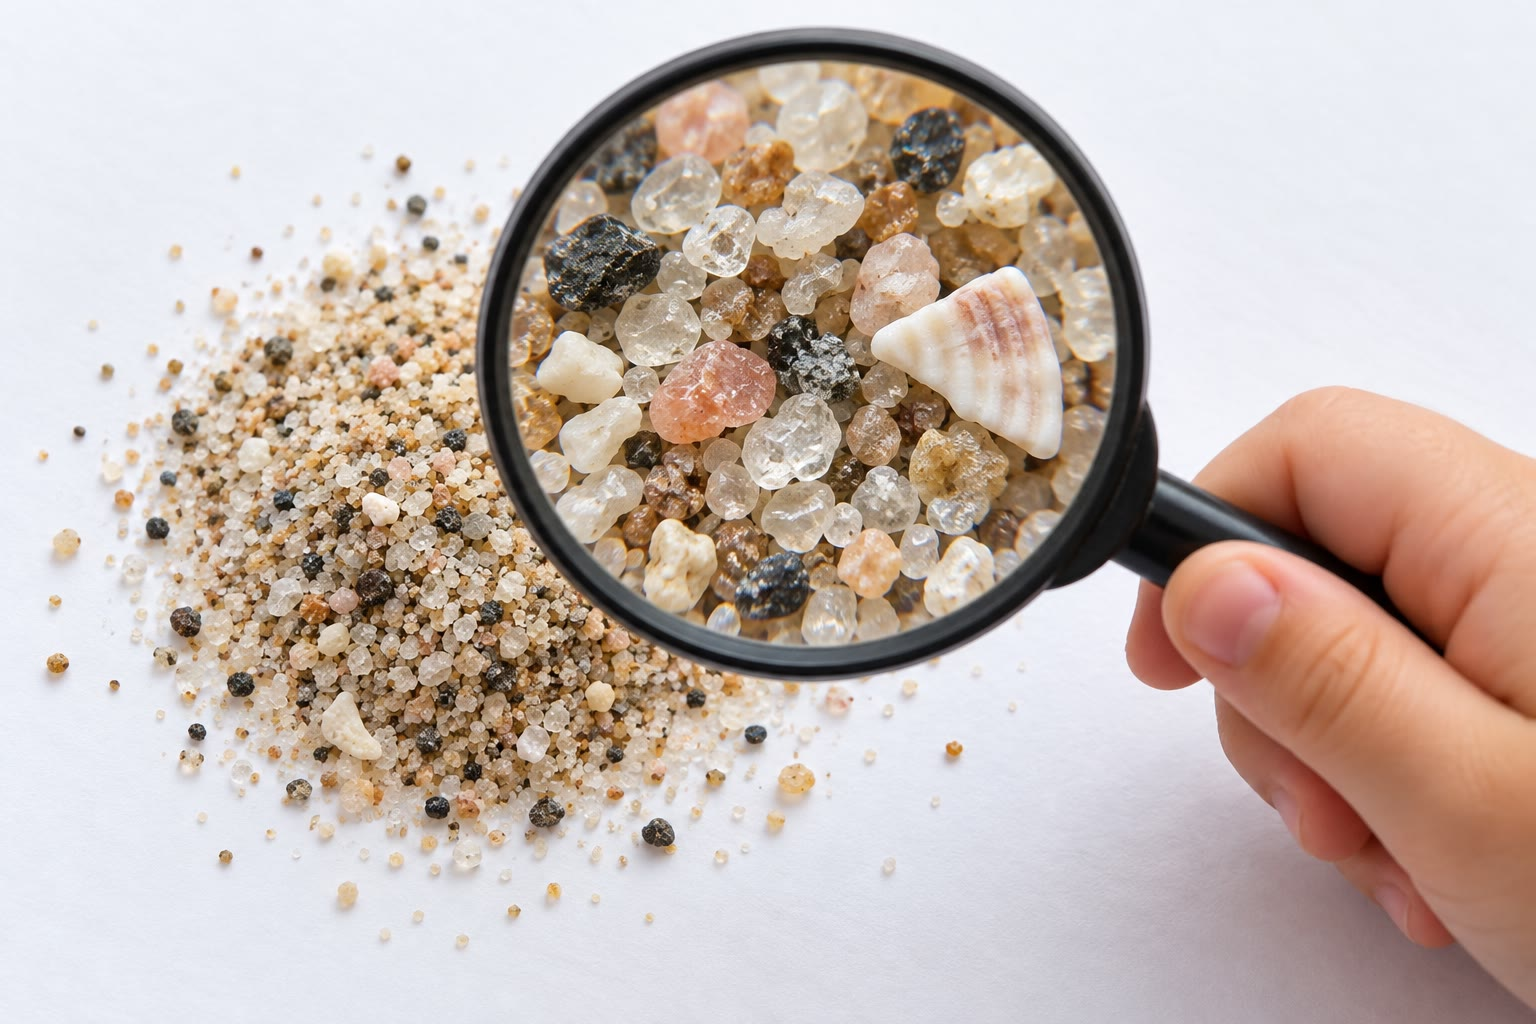
\includegraphics[width=0.55\linewidth]{images/book1/ai/g3-sand-magnifier.jpg}

{\small \omterm{def:g3:stones-pebbles-sand:sand}{Pasir} pantai yang dilihat dengan kaca pembesar: butiran-butiran
\omterm{def:g3:stones-pebbles-sand:rock}{batuan} yang sangat kecil dan potongan-potongan cangkang.}
\end{omfigure}

\begin{method}[Memilah pecahan batuan menurut ukuran]\label{met:g3:stones-pebbles-sand:sort}
Untuk menamai sepotong pecahan \omterm{def:g3:stones-pebbles-sand:rock}{batuan}, perhatikan ukurannya:
\begin{enumerate}
  \item jika kamu tidak bisa melihat butirannya, bahkan dari dekat, itulah
        \omterm{def:g3:stones-pebbles-sand:sand}{lumpur};
  \item jika kamu bisa melihat setiap butir, tetapi setiap butir lebih kecil
        daripada 2 milimeter (setebal sekeping uang logam), itulah \omterm{def:g3:stones-pebbles-sand:sand}{pasir};
  \item jika potongannya lebih besar daripada itu, tetapi kamu bisa
        menggenggam satu di tanganmu, itulah \omterm{def:g3:stones-pebbles-sand:pebble}{kerikil} dan \omterm{def:g3:stones-pebbles-sand:pebble}{kerakal};
  \item jika sepotong terlalu berat untuk diangkat, itulah bongkah.
\end{enumerate}
\end{method}

\begin{example}[Di mana kita menemukan setiap ukuran?]\label{ex:g3:stones-pebbles-sand:where}
Air yang deras bisa membawa batu-batu besar; air yang lambat menjatuhkannya
dan hanya membawa butiran kecil. Jadi bongkah dan batu tajam terletak di
\omterm{def:g1:landscapes-around-us:water}{sungai-sungai} kecil pegunungan yang curam; \omterm{def:g3:stones-pebbles-sand:pebble}{kerakal} dan \omterm{def:g3:stones-pebbles-sand:pebble}{kerikil} terletak di
tepi \omterm{def:g1:landscapes-around-us:water}{sungai} di \omterm{def:g1:landscapes-around-us:landform}{lembah}; \omterm{def:g3:stones-pebbles-sand:sand}{pasir} berkumpul di pantai dan di kelokan \omterm{def:g1:landscapes-around-us:water}{sungai} yang
tenang; dan \omterm{def:g3:stones-pebbles-sand:sand}{lumpur} mengendap di tempat airnya hampir diam, di kolam, di
\omterm{def:g1:landscapes-around-us:water}{danau}, dan di muara \omterm{def:g1:landscapes-around-us:water}{sungai}.
\end{example}

\section{Batuan keras dan batuan lunak}

Tidak semua \omterm{def:g3:stones-pebbles-sand:rock}{batuan} sama kerasnya. Sebagian, seperti granit, begitu keras
sehingga bisa menggores kaca dan bertahan ribuan tahun di dalam dinding.
Sebagian lain hancur di tangan, seperti kapur, yang meninggalkan bekas putih
di papan. Sebagian \omterm{def:g3:stones-pebbles-sand:rock}{batuan} tersusun dari butiran yang bisa kita lihat;
sebagian lain halus dan tampak sama saja dari satu sisi ke sisi yang lain.

\begin{example}[Tiga batuan dibandingkan]\label{ex:g3:stones-pebbles-sand:three}
\emph{Granit} berbintik-bintik dengan butiran merah muda, putih, dan hitam,
dan sangat keras. \emph{Batu pasir} tersusun dari butiran \omterm{def:g3:stones-pebbles-sand:sand}{pasir} yang saling
melekat; jika digosok dengan jari, kadang-kadang beberapa butirnya lepas.
\emph{Kapur} berwarna putih, lunak, dan seperti bubuk. Di tahun berikutnya
kamu akan mempelajari bagaimana masing-masing \omterm{def:g3:stones-pebbles-sand:rock}{batuan} itu terbentuk.
\end{example}

\begin{omfigure}
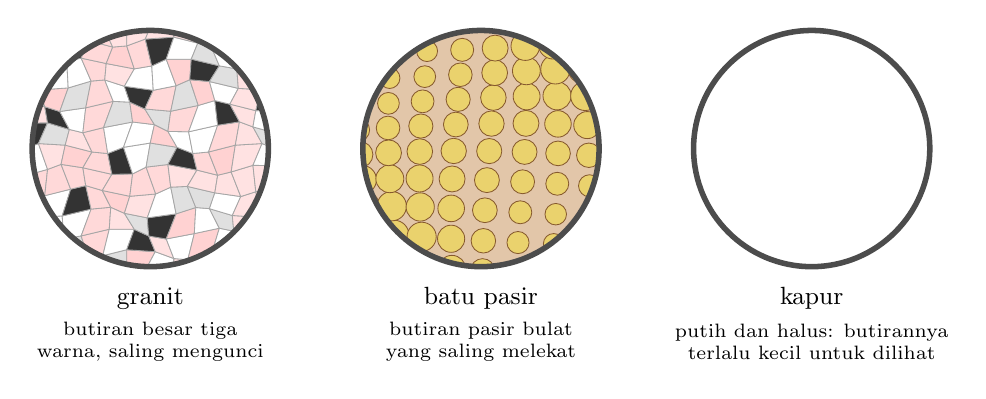
\begin{tikzpicture}[font=\small]
  % three stones seen through a magnifying glass (drawn, not to scale)
  % granite: interlocking grains of three colours
  \begin{scope}
    \clip (0,0) circle (1.5);
    % a jittered lattice: the cells tile the disk with no gap, like the
    % interlocking crystals of granite
    \foreach \i in {-6,...,5} \foreach \j in {-6,...,5} {
      \pgfmathtruncatemacro{\c}{mod(abs(37*\i+17*\j+\i*\j),7)}
      \ifcase\c \def\col{pink!70}\or\def\col{pink!45}\or\def\col{white}\or
        \def\col{black!12}\or\def\col{white}\or\def\col{black!80}\else\def\col{pink!60}\fi
      \fill[\col, draw=black!35, line width=0.3pt]
        ({0.27*\i+0.07*sin(90*\i+131*\j)},{0.27*\j+0.07*cos(77*\i+61*\j)}) --
        ({0.27*(\i+1)+0.07*sin(90*(\i+1)+131*\j)},{0.27*\j+0.07*cos(77*(\i+1)+61*\j)}) --
        ({0.27*(\i+1)+0.07*sin(90*(\i+1)+131*(\j+1))},{0.27*(\j+1)+0.07*cos(77*(\i+1)+61*(\j+1))}) --
        ({0.27*\i+0.07*sin(90*\i+131*(\j+1))},{0.27*(\j+1)+0.07*cos(77*\i+61*(\j+1))}) -- cycle;
    }
  \end{scope}
  \draw[black!70, line width=2pt] (0,0) circle (1.5);
  \node at (0,-1.9) {granit};
  \node[font=\scriptsize, align=center] at (0,-2.45) {butiran besar tiga\\warna, saling mengunci};
  % sandstone: rounded grains touching
  \begin{scope}[xshift=4.2cm]
    \clip (0,0) circle (1.5);
    \fill[brown!45] (-1.6,-1.6) rectangle (1.6,1.6);
    \foreach \x in {-1.5,-1.1,...,1.6} \foreach \y in {-1.5,-1.15,...,1.6}
      \fill[yellow!50!brown!70, draw=brown!70!black, line width=0.3pt]
        ({\x+0.08*sin(97*\x+61*\y)},{\y+0.07*cos(53*\x-89*\y)}) circle ({0.16+0.03*sin(71*\x*\y)});
  \end{scope}
  \draw[black!70, line width=2pt] (4.2,0) circle (1.5);
  \node at (4.2,-1.9) {batu pasir};
  \node[font=\scriptsize, align=center] at (4.2,-2.45) {butiran pasir bulat\\yang saling melekat};
  % chalk: smooth, no grains to see
  \begin{scope}[xshift=8.4cm]
    \fill[white] (0,0) circle (1.5);
  \end{scope}
  \draw[black!70, line width=2pt] (8.4,0) circle (1.5);
  \node at (8.4,-1.9) {kapur};
  \node[font=\scriptsize, align=center] at (8.4,-2.45) {putih dan halus: butirannya\\terlalu kecil untuk dilihat};
\end{tikzpicture}

{\small Tiga \omterm{def:g3:stones-pebbles-sand:rock}{batuan} yang dilihat dengan kaca pembesar (digambar). Butiran
granit dan batu pasir dapat dilihat; kapur tampak sama di semua bagiannya.}
\label{fig:g3:stones-pebbles-sand:magnified}
\end{omfigure}

\begin{method}[Mengamati batu dari dekat]\label{met:g3:stones-pebbles-sand:look}
Untuk menggambarkan sebuah batu, lihatlah dan rabalah batu itu, tanpa
memecahkannya:
\begin{enumerate}
  \item warnanya, atau warna-warnanya;
  \item bentuknya: tajam dan bersudut, atau bulat dan licin;
  \item butirannya: dapatkah kamu melihatnya? apakah semuanya sama, atau
        terdiri atas beberapa warna?
  \item rasanya saat diraba: keras, atau cukup lunak untuk meninggalkan
        bekas di kertas?
\end{enumerate}
Tuliskan apa yang kamu lihat dalam sebuah tabel, satu baris untuk setiap batu.
\end{method}

\begin{example}[Tabel tiga batu]\label{ex:g3:stones-pebbles-sand:table}
Mia menggambarkan tiga batu dari sebuah kotak di sekolah.
\begin{center}\small
\begin{tabular}{llll}
\hline
Batu & Warna & Bentuk & Butiran \\
\hline
A & merah muda, putih, dan hitam & bulat & besar, tiga warna \\
B & kuning kecokelatan & tajam & kecil, semuanya serupa \\
C & putih & tajam & tidak terlihat \\
\hline
\end{tabular}
\end{center}
Batu C juga meninggalkan bekas putih di kertas. Menurut contoh di atas,
batu A mirip granit, batu B mirip batu pasir, dan batu C mirip kapur.
Batu A bulat: air sudah lama menggulingkannya.
\end{example}

\section{Batu yang kita pakai untuk membangun}

Selama ribuan tahun, manusia membangun dengan \omterm{def:g3:stones-pebbles-sand:rock}{batuan} di sekitar mereka. Di
desa-desa tua di suatu daerah, dinding-dindingnya sering berwarna sama
semua, karena dibangun dengan batu dari \omterm{def:g1:landscapes-around-us:landform}{bukit} yang paling dekat.

\begin{definition}[Batu bangunan]\label{def:g3:stones-pebbles-sand:building-stone}
Yang disebut \emph{batu bangunan}\index{batu bangunan} adalah \omterm{def:g3:stones-pebbles-sand:rock}{batuan} yang
dipotong atau dibentuk untuk membangun dinding, atap, anak tangga,
jembatan, atau trotoar.
\end{definition}

Setiap \omterm{def:g3:stones-pebbles-sand:rock}{batuan} cocok untuk sesuatu. Granit yang keras dijadikan dinding,
anak tangga, dan batu tepi jalan yang bertahan berabad-abad. Sebagian
\omterm{def:g3:stones-pebbles-sand:rock}{batuan}, seperti batu sabak, terbelah menjadi lembaran yang tipis dan
datar: jika disusun saling menindih, lembaran itu menjadi atap yang
menahan hujan. Batu pasir dan batu kapur cukup lunak untuk dipotong
menjadi balok-balok yang rapi.

\begin{omfigure}
\begin{minipage}[b]{0.49\linewidth}\centering
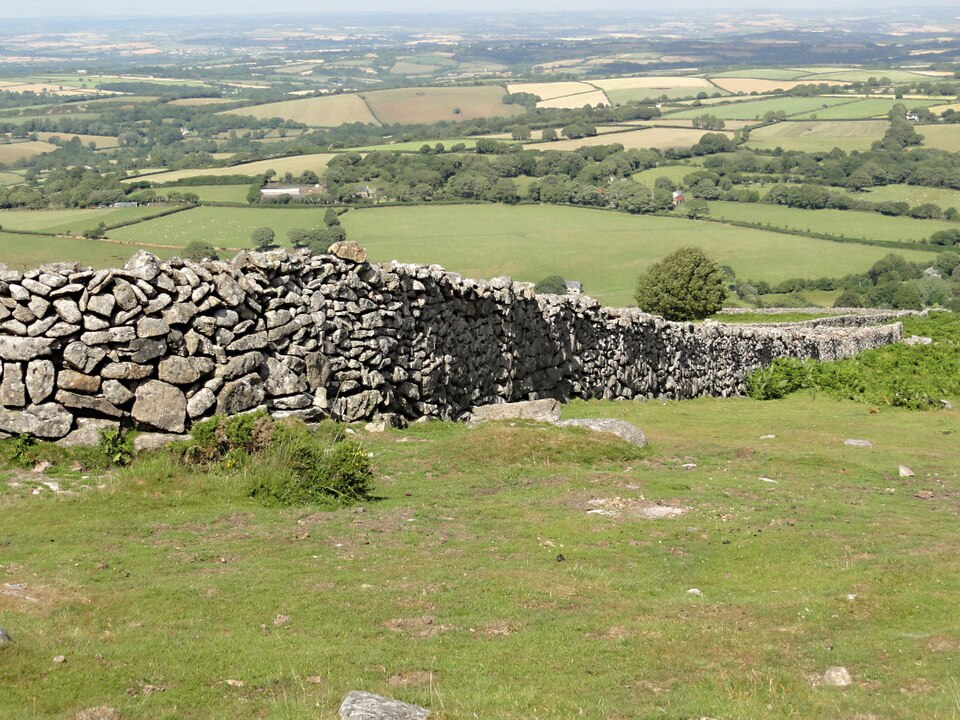
\includegraphics[width=\linewidth]{images/book1/g3-granite-wall.jpg}

{\small Dinding dari balok-balok granit, dibangun tanpa adukan semen.
Foto: Tony Atkin, Geograph (CC BY-SA 2.0).}
\end{minipage}\hfill
\begin{minipage}[b]{0.49\linewidth}\centering
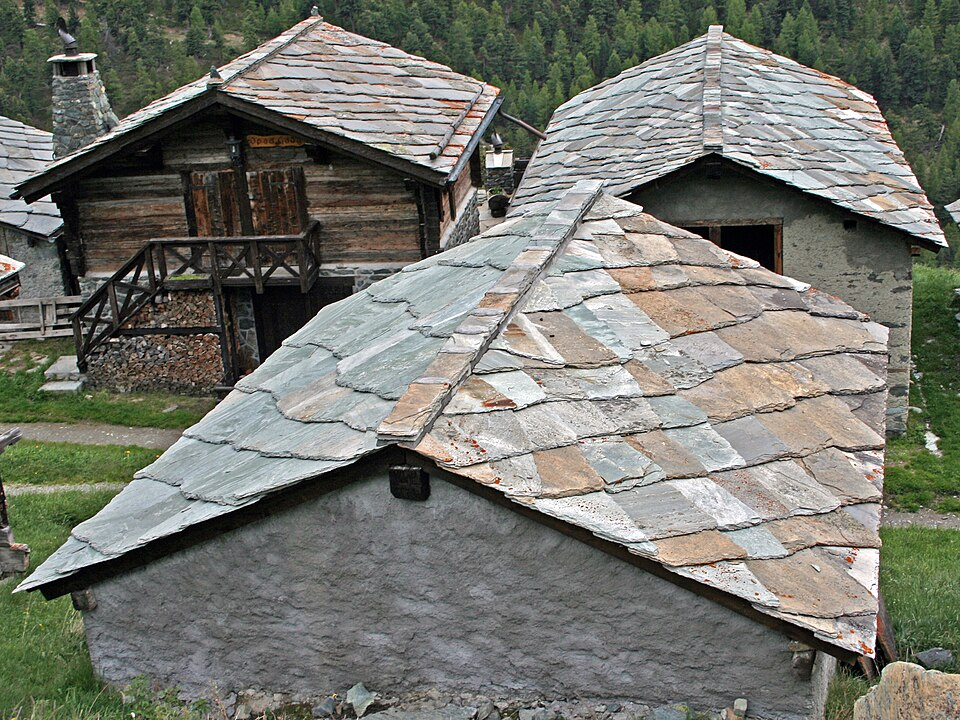
\includegraphics[width=\linewidth]{images/book1/g3-slate-roof.jpg}

{\small Atap dari lempengan batu yang tipis dan datar di sebuah desa
pegunungan di Swiss. Foto: Michael C. Rygel (CC BY-SA 3.0).}
\end{minipage}
\end{omfigure}

\begin{omfigure}
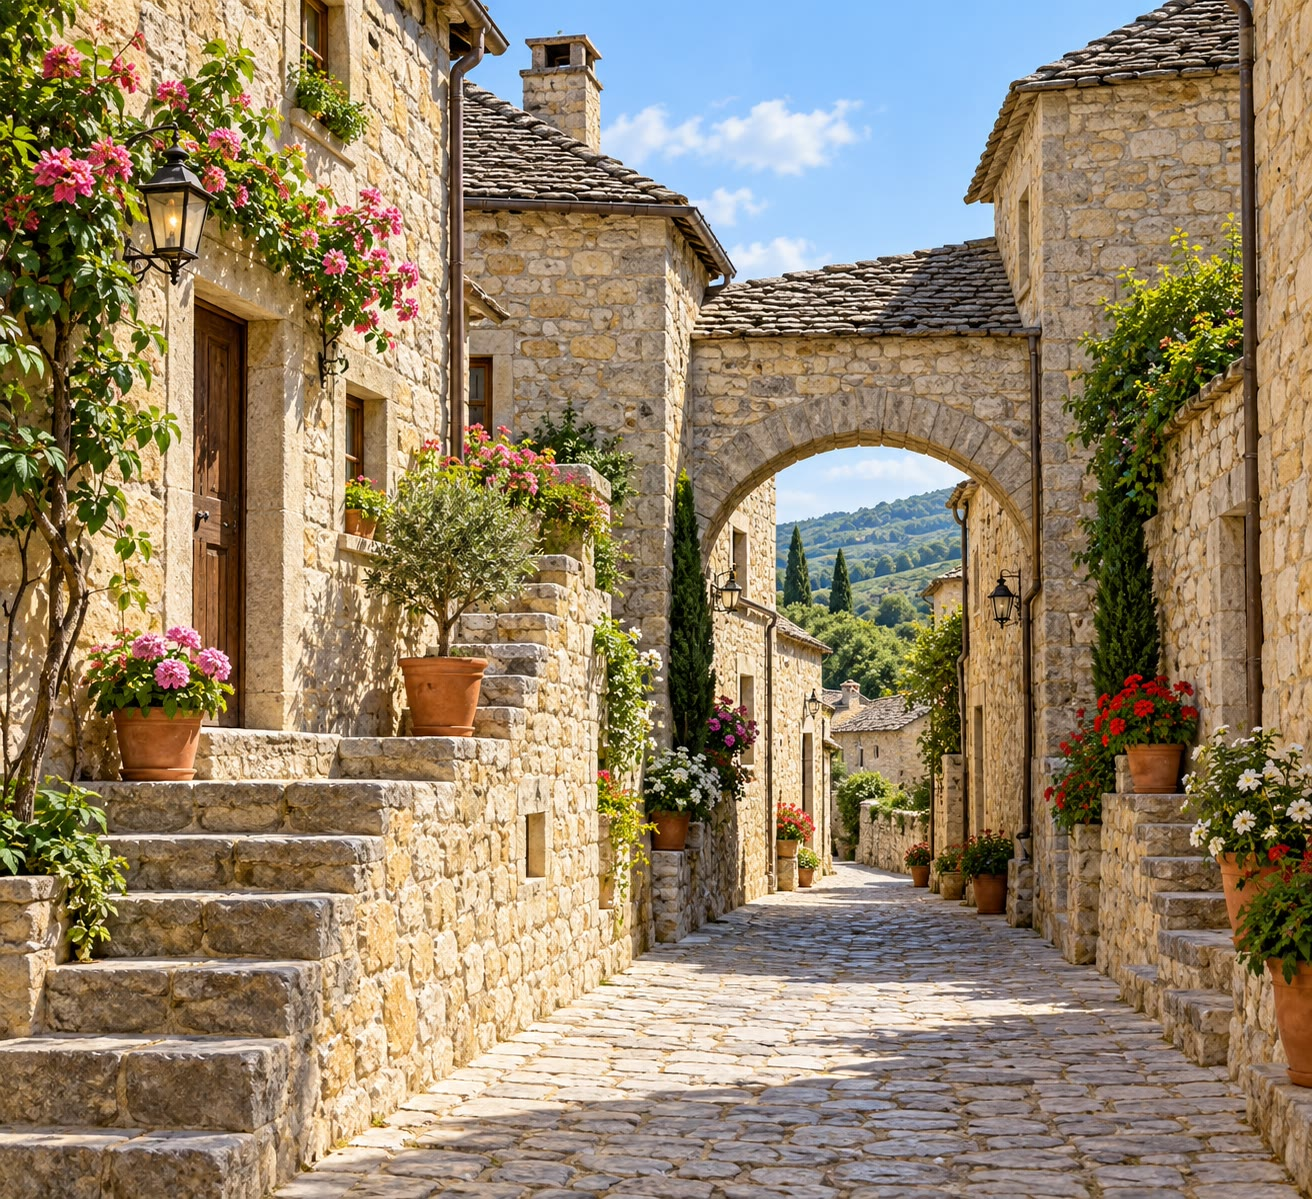
\includegraphics[width=0.6\linewidth]{images/book1/ai/g3-stone-village.jpg}

{\small Desa tua yang seluruhnya dibangun dengan batu dari \omterm{def:g1:landscapes-around-us:landform}{bukit} di dekatnya.}
\end{omfigure}

Sekarang kita juga membangun dengan bata, beton, dan kaca. Tetapi bata
dibuat dari tanah liat yang dibakar, beton dibuat dari \omterm{def:g3:stones-pebbles-sand:sand}{pasir}, \omterm{def:g3:stones-pebbles-sand:pebble}{kerikil}, dan
semen, dan kaca dibuat dari \omterm{def:g3:stones-pebbles-sand:sand}{pasir}: semuanya juga berasal dari \omterm{def:g3:stones-pebbles-sand:rock}{batuan} Bumi.

\section{Latihan}

\begin{exercise}[$\star$]\label{exo:g3:stones-pebbles-sand:1}
Apa itu \omterm{def:g3:stones-pebbles-sand:rock}{batuan dasar}? Di mana kita bisa melihatnya tanpa menggali?
\end{exercise}

\begin{exercise}[$\star$]\label{exo:g3:stones-pebbles-sand:2}
Urutkan menurut ukurannya, dari yang terkecil sampai yang terbesar:
\omterm{def:g3:stones-pebbles-sand:pebble}{kerakal}, \omterm{def:g3:stones-pebbles-sand:sand}{lumpur}, bongkah, \omterm{def:g3:stones-pebbles-sand:sand}{pasir}.
\end{exercise}

\begin{exercise}[$\star$]\label{exo:g3:stones-pebbles-sand:3}
Sebutir butiran berukuran 1 milimeter. Apakah butiran itu \omterm{def:g3:stones-pebbles-sand:sand}{pasir} atau
\omterm{def:g3:stones-pebbles-sand:pebble}{kerikil}? Butiran lain berukuran 3 milimeter: \omterm{def:g3:stones-pebbles-sand:sand}{pasir} atau \omterm{def:g3:stones-pebbles-sand:pebble}{kerikil}?
\end{exercise}

\begin{exercise}[$\star$]\label{exo:g3:stones-pebbles-sand:4}
Alami atau buatan manusia? \omterm{def:g3:stones-pebbles-sand:pebble}{Kerakal}; bata; balok granit; selembar kaca;
\omterm{def:g3:stones-pebbles-sand:sand}{pasir} di pantai.
\end{exercise}

\begin{exercise}[$\star$]\label{exo:g3:stones-pebbles-sand:5}
Mengapa \omterm{def:g3:stones-pebbles-sand:pebble}{kerakal} dari \omterm{def:g1:landscapes-around-us:water}{sungai} tidak mempunyai sudut yang tajam?
\end{exercise}

\begin{exercise}[$\star$]\label{exo:g3:stones-pebbles-sand:6}
Sebutkan dua \omterm{def:g3:stones-pebbles-sand:building-stone}{batu bangunan} dan katakan untuk apa masing-masing dipakai
pada foto-foto di bab ini.
\end{exercise}

\begin{exercise}[$\star\star$]\label{exo:g3:stones-pebbles-sand:7}
Tom menemukan dua batu dari \omterm{def:g3:stones-pebbles-sand:rock}{batuan} yang sama: yang satu tajam, yang lain
bulat. Batu mana yang sudah menempuh perjalanan lebih jauh? Jelaskan.
\end{exercise}

\begin{exercise}[$\star\star$]\label{exo:g3:stones-pebbles-sand:8}
Pada gambar ukuran butiran, berapa sentimeter panjang \omterm{def:g3:stones-pebbles-sand:pebble}{kerakal} yang terbesar?
Berapa butir \omterm{def:g3:stones-pebbles-sand:sand}{pasir} berukuran 2 milimeter yang muat berjajar sepanjang 1
sentimeter?
\end{exercise}

\begin{exercise}[$\star\star$]\label{exo:g3:stones-pebbles-sand:9}
Di mana kamu akan menduga menemukan \omterm{def:g3:stones-pebbles-sand:sand}{lumpur}: di \omterm{def:g1:landscapes-around-us:water}{sungai} kecil pegunungan yang
deras atau di kolam yang tenang? Mengapa?
\end{exercise}

\begin{exercise}[$\star\star$]\label{exo:g3:stones-pebbles-sand:10}
Bata, beton, dan kaca dibuat oleh manusia. Mengapa kita tetap bisa
mengatakan bahwa semuanya berasal dari \omterm{def:g3:stones-pebbles-sand:rock}{batuan} Bumi?
\end{exercise}
